\chapter{Introduction (Incomplete)}\label{ch-introduction}
\thispagestyle{headings}
\markboth{Chapter \ref{ch-introduction}: Introduction}{Chapter \ref{ch-introduction}: Introduction}

%The purpose of this chapter is to introduce the main concepts and results necessary for
%a more formal treatment of the prediction problem.
%Section \ref{sc-intro-qoi} presents a first mathematical model of a system, as well as the applicability of Bayes' theorem to our prediction problem.
%The chapter finishes with the presentation of a more detailed model of a system in Section \ref{sc-intro-detail}.

The QUESO library is able to handle uni- and multi-processor Linux
environments.

%Other docs: \cite{PrSc09} and html.

\section{Key Statistical Concepts}


Inverse problems are defined as the inverse of direct or forward problems, as the term itself suggests.
Inverse problems apply, in general, to situations were certain quantities of interest are different from the ones that are accessible to measurements \cite{Andersen2001}. 

% A typical feature of inverse problems is that they often fail to fulfill Hadamard's presumptions of well-posedness, i.e., a unique solution may not exist or may not depend continuously  on the given data.
% By reformulating inverse problems for statistical inference,  regularization of ill-posed problems may be obtained through Bayesian approach ( 
% by assuming that the a priori beliefs about the solution before having observed any data can be described by a prior distribution). 

% Statistical inverse theory reformulates inverse problems as problems of statistical inference by means of Bayesian statistics. In Bayesian statistics all quantities are modeled as random variable. The randomness, which reflects the observer's uncertainty concerning their values, is coded in the probability distribution of the quantities. From the perspective of statistical inversion theory, the solution to an inverse problem is the probability distribution of the quantity of interest when all information available has been incorporated in the model. This distribution, called the posterior distribution, describes the degree of confidence about the quantity after the measurement has been performed.

Statistical inverse theory reformulates inverse problems as problems of statistical inference by means of Bayesian statistics: all quantities are modeled as random variables, and probability distribution of the quantities encapsulates the uncertainty observed in their values. The solution to the inverse problem is then the probability distribution of the quantity of interest when all information available has been incorporated in the model. This (posterior) distribution describes the degree of confidence about the quantity after the measurement has been performed \cite{KaSo05}.

Thus, the solution to the statistical inverse problem may be given by Bayes' formula, which express the posterior distribution as a function of the prior distribution and the data represented through the likelihood function.

The likelihood function has an open-form and its evaluation is highly computer intensive.  Moreover, simulation-based posterior inference requires a large number of forward calculations to be performed, therefore, fast and efficient sampling techniques are required for posterior inference.

It is often not straightforward to obtain explicit posterior point estimates of the solution, since it usually involves the evaluation of a high-dimensional integral with respect to a possibly non-smooth posterior distribution. In such cases, an alternative integration technique is the Markov chain Monte Carlo method: posterior means may be estimated using the sample mean from a series of random draws from the posterior distribution.

QUESO library provides tools for sampling algorithms for statistical inverse problems, following Bayes' formula, and statistical forward problems. It contains Monte Carlo solvers, MCMC (e.g. Metropolis Hastings \cite{Metr_1953,Hast_1970}) as well as the DRAM \cite{HaLaMiSa06}; it also has the capacity to handle many chains or sequences in parallel, each chain or sequence itself demanding many computing nodes because of the computational model being statistically explored \cite{PrSc09}.


A computational model is a combination of a
mathematical model and a discretization that enables the approximate
solution of the mathematical model using computer algorithms and  might be used in two different types of problems:
forward or inverse. 

Any computational model is composed of a vector $\boldsymbol{\theta}$ of $n$ {\it parameters}, {\it state variables} $\mathbf{u}$, and {\it state equations} $\mathbf{r}(\boldsymbol{\theta},\mathbf{u}) = \mathbf{0}$.
Once the solution $\mathbf{u}$ is available, the computational model also includes extra functions for e.g.
the calculation of {\it model output data} $\mathbf{y} = \mathbf{y}(\boldsymbol{\theta},\mathbf{u})$, and the {\it prediction} of a
vector $\mathbf{q} = \mathbf{q}(\boldsymbol{\theta},\mathbf{u})$ of $m$~quantities~of~interest\text{ (QoI)},

Parameters designate all model variables that are neither state variables
nor further quantities computed by the model, such as: material properties, coefficients, constitutive parameters, boundary conditions, initial conditions,
external forces, parameters for modeling the model error, characteristics of an experimental apparatus (collection of devices and procedures),
discretization choices and numerical algorithm options.

% Some parameters might be directly measurable, e.g. room temperature,
% but some may not, e.g. a material property.
% Parameters that cannot be measured directly need to be {\it estimated}
% through the solution of an {\it inverse problem}.


In the case of a forward problem, the parameters $\boldsymbol{\theta}$ are given and
one then needs to compute $\mathbf{u}$, $\mathbf{y}$ and/or $\mathbf{q}$.
In the case of an inverse problem, however, experimental data $\mathbf{d}$ is given and
one then needs to {\it estimate} the values of the parameters $\boldsymbol{\theta}$ that
cause $\mathbf{y}$ to best fit  $\mathbf{d}$.
%where ``best'' is an algorithm dependent concept.

%The process of parameter estimation is also referred to as model calibration or model update, and it usually precedes the computation of a QoI, a process called model prediction. 

Figure~\ref{fig-generic-problems} represents general inverse and forward problems respectively.
\begin{figure}[htbp]
\vspace{-10pt}
\begin{center}
% \subfigure[]{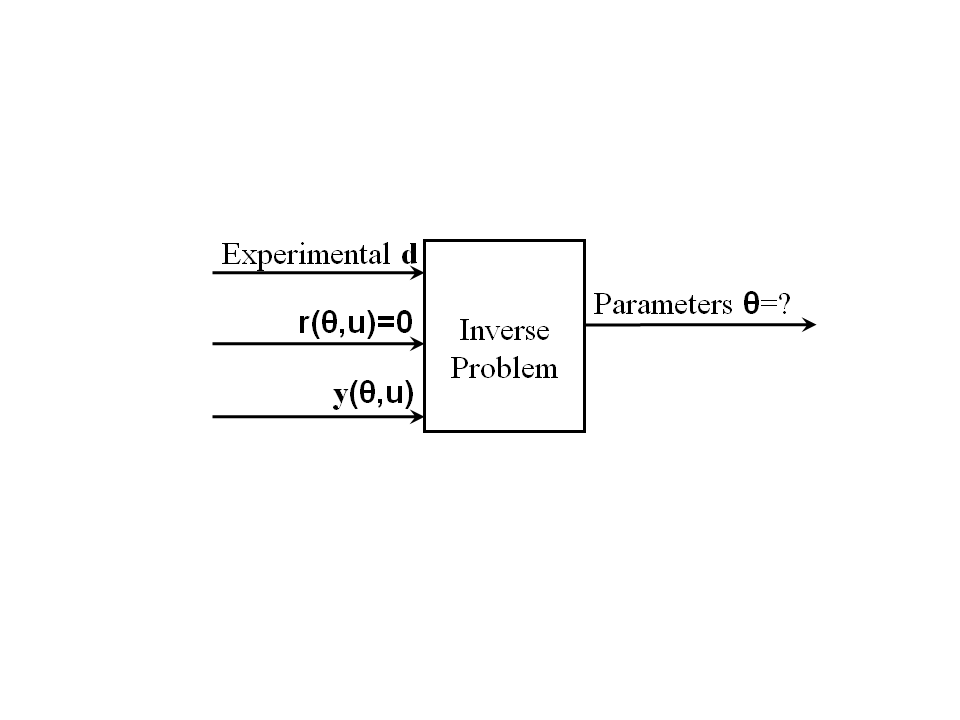
\includegraphics[scale=0.50,clip=true,viewport=1.7in 3.0in 8.5in 5.5in]{figs/queso_paper1_08.png}}
% \subfigure[]{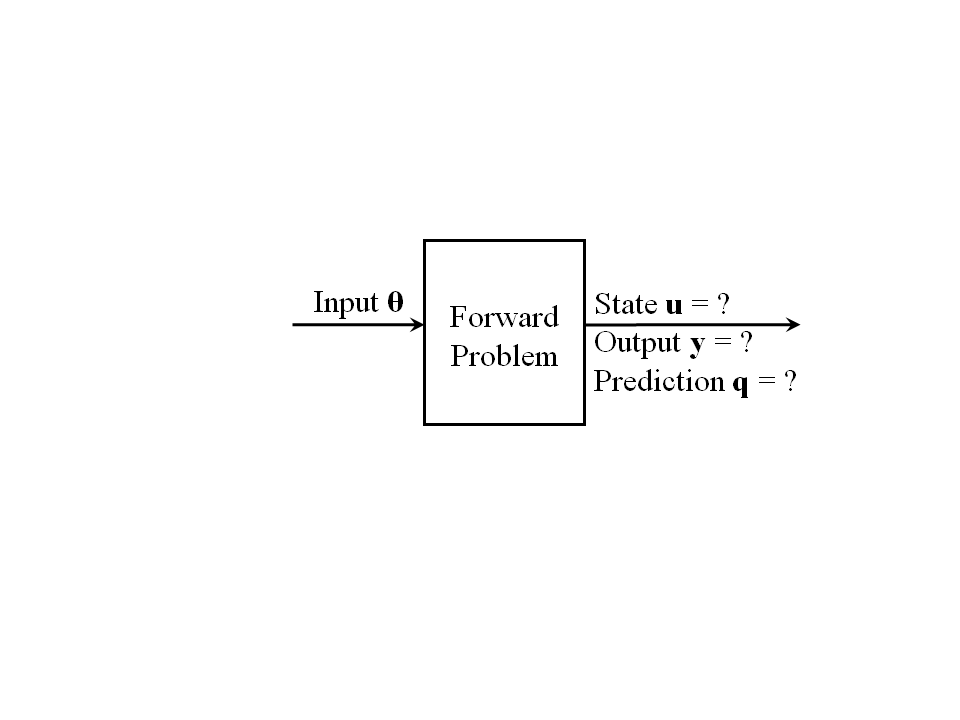
\includegraphics[scale=0.50,clip=true,viewport=1.8in 3.0in 8.4in 5.5in]{figs/queso_paper1_07.png}}
\subfigure[]{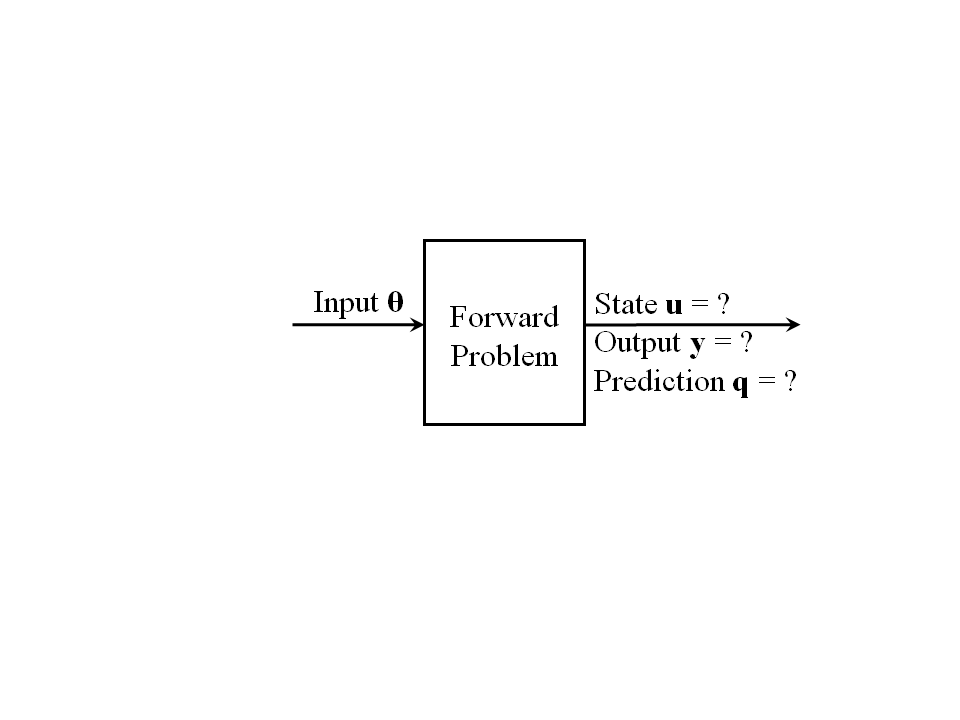
\includegraphics[scale=0.45,clip=true,viewport=1.9in 3.0in 8.5in 5.5in]{figs/queso_paper1_07.png}}\quad\quad
\subfigure[]{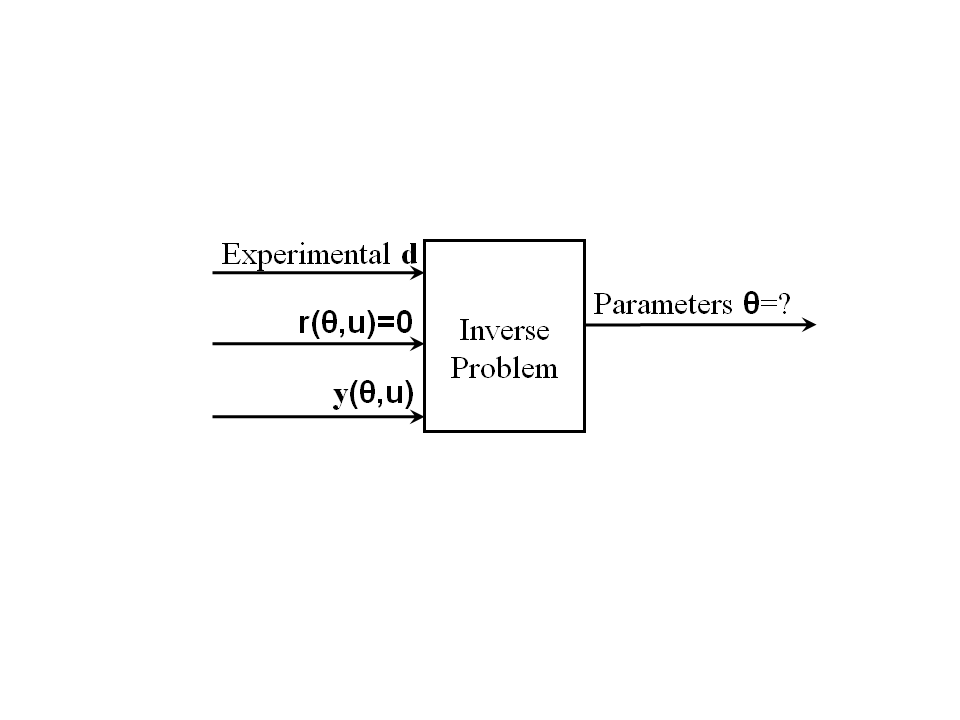
\includegraphics[scale=0.45,clip=true,viewport=1.9in 3.0in 8.5in 5.5in]{figs/queso_paper1_08.png}}
\end{center}
\vspace{-20pt}
\caption{The representation of (a) a generic forward problem and (b) a generic inverse problem.}
\label{fig-generic-problems}
\end{figure}



There are many possible sources of uncertainty on a computational model. %procedures (a) and (b) above. 
First, $\mathbf{d}$ need not be equal to the actual values of observables because of errors in the measurement process. Second, the values of the input parameters to the phenomenon might not be precisely known. Third, the appropriate set of
equations governing the phenomenon might not be well understood. 

Computational models can be classified as either deterministic or stochastic -- which are the ones of interest here.  In deterministic models, all parameters are assigned numbers, and no parameter is related to the parametrization of a random variable (RV) or field. As a
consequence, a deterministic model assigns a number to each of the components of quantities $\mathbf{u}$, $\mathbf{y}$ and $\mathbf{q}$. In stochastic models, however, at least one parameter is assigned a probability density function (PDF) or is related to the parametrization of a RV or field, causing $\mathbf{u}$, $\mathbf{y}$ and $\mathbf{q}$ to become random variables.  Note that not all components of $\boldsymbol{\theta}$ need to be treated as random. As long as at least one component is random, $\boldsymbol{\theta}$ is a random vector, and the problem is stochastic.



In the case of forward problems, statistical forward problems can be represented very similarly to deterministic forward problems,
as seen in Figure \ref{fig-sfp-queso}.
In the case of inverse problems, as depicted in Figure \ref{fig-sip-queso}, however, the conceptual connection between deterministic and statistical problems
is not as straightforward.

\begin{figure}[h!]
\centerline{
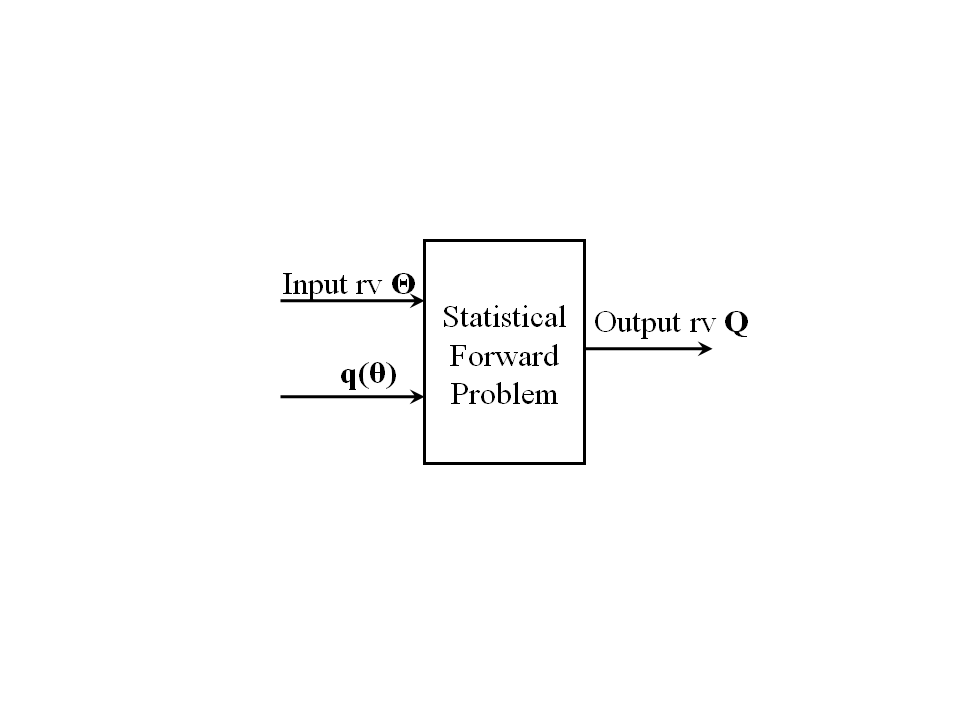
\includegraphics[scale=0.45,clip=true,viewport=1.0in 2.5in 10.0in 5.5in]{figs/queso_paper1_09}
}
\caption{
The representation of a statistical forward problem.
$\boldsymbol{\Theta}$ denotes a random variable related to parameters,
$\boldsymbol{\theta}$ denotes a realization of $\boldsymbol{\Theta}$ and
$\mathbf{Q}$ denotes a random variable related to quantities of interest.
}
\label{fig-sfp-queso}
\end{figure}

\begin{figure}[h!]
\centerline{
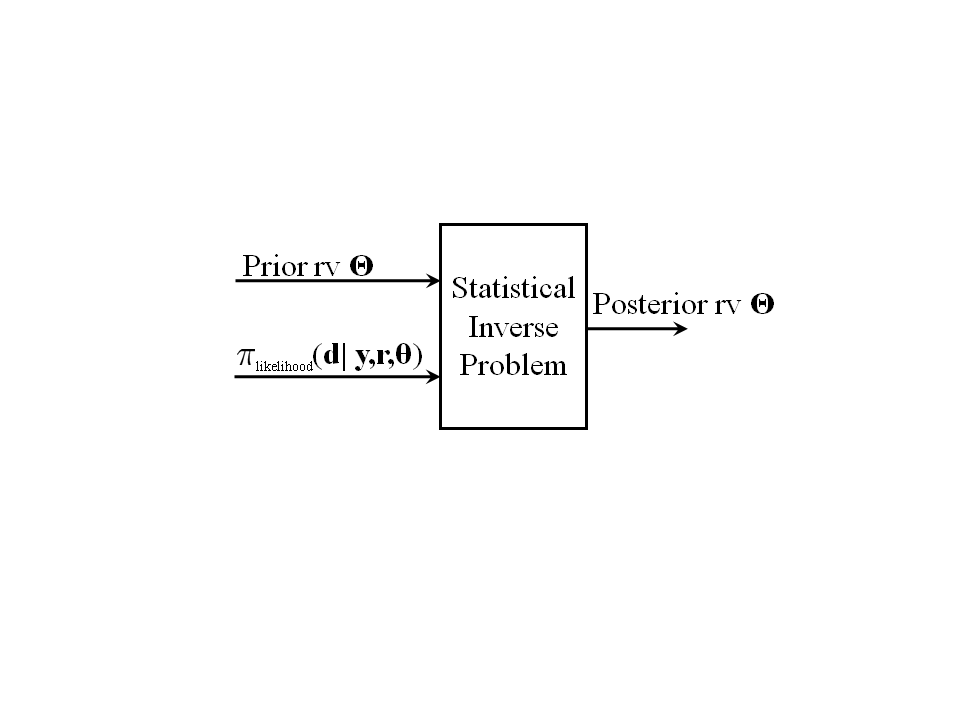
\includegraphics[scale=0.45,clip=true,viewport=1.0in 3.0in 10.0in 5.5in]{figs/queso_paper1_10}
}
\caption{
The representation of a statistical inverse problem.
$\boldsymbol{\Theta}$ denotes a random variable related to parameters,
$\boldsymbol{\theta}$ denotes a realization of $\boldsymbol{\Theta}$ and
$\mathbf{r}$ denotes model equations,
$\mathbf{y}$ denotes some model output data and
$\mathbf{d}$ denotes experimental data.
}
\label{fig-sip-queso}
\end{figure}


QUESO adopts a Bayesian analysis \cite{KaSo05, Ro04} for statistical inverse problems, interpreting the posterior PDF
\begin{equation}\label{eq-Bayes-solution}
\pi_{\text{posterior}}(\boldsymbol{\theta}|\mathbf{d})=\frac{\pi_{\text{prior}}(\boldsymbol{\theta})\pi_{\text{likelihood}}(\mathbf{d}|\boldsymbol{\theta})}{\pi(\mathbf{d})}
\end{equation}
as the solution. Such solutions combine the prior information $\pi_{\text{prior}}(\boldsymbol{\theta})$ of the parameters,
the information $\pi(\mathbf{d})$ on the data, and the likelihood $\pi_{\text{likelihood}}(\mathbf{d}|\boldsymbol{\theta})$ that the model computes certain data values with a given set of input parameters.

This semantic interpretation of achieving a posterior knowledge on the parameters (on the model)
after combining some prior model knowledge with experimental information provides an important mechanism for dealing with uncertainty.
Although mathematically simple, is not computationally trivial. 


\section{The Software Stack of an Application Using QUESO}

\begin{figure}[h!]
\centerline{
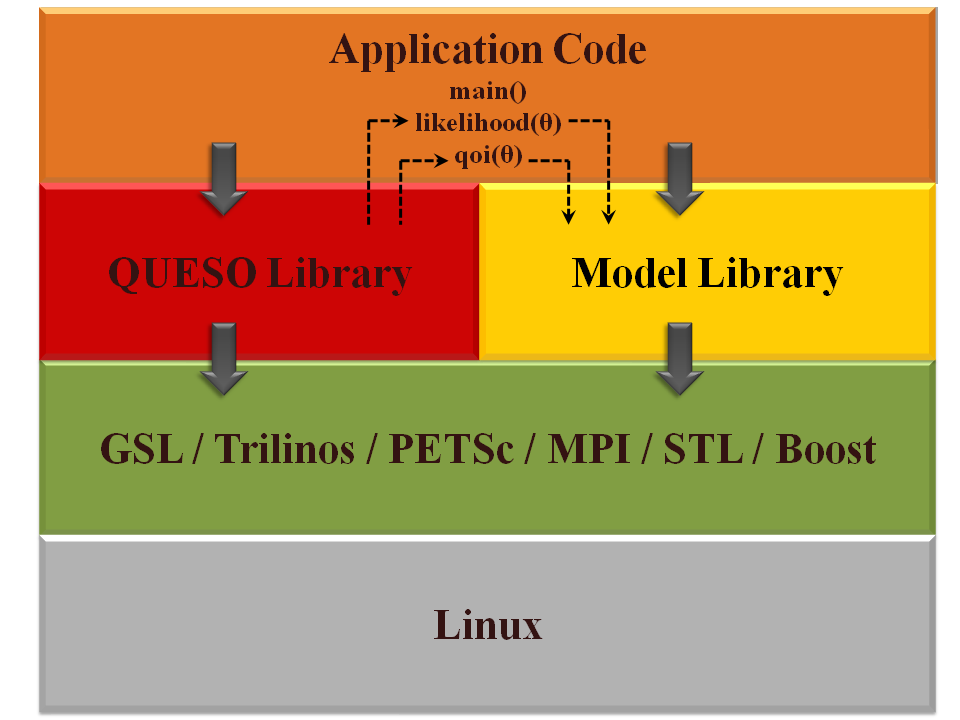
\includegraphics[scale=0.50,clip=true]{figs/queso_paper1_03}
}
\caption{
Overview of the software stack of a typical application that uses QUESO.
The symbol $\boldsymbol{\theta}$ represents a vector of $n\geqslant 1$ parameters.
Algorithms in the QUESO library require the supply
of a likelihood routine $\pi_{\text{like}}:\mathbb{R}^n\rightarrow\mathbb{R}_+$ for statistical inverse problems and 
of a qoi routine $\mathbf{q}:\mathbb{R}^n\rightarrow\mathbb{R}^m$ for statistical forward problems. These routines
exist at the application level and provide the necessary bridge between the statistical algorithms in QUESO,
model knowledge in the model library and scenario and experimental data in the disk space.
Concepts are further detailed in Chapter \ref{ch-introduction}.
}
\label{fig-sw-stack}
\end{figure}

\subsection{A QUESO Environment}

\subsection{Using Other C++ Classes in the Library}

\subsection{Input and Output Files}

